\section{\secondtitle}

\begin{frame}
\frametitle{\textbf{Predicting learned-cuts}}
 
  \onslide<1->{
  % \begin{block}{Given an optimization problem}
  %   \begin{equation*}
  %     y^{*}(x) :\equiv arg \,\,\min_{y \in \mathcal{Y}(x)} C(x,y)
  %   \end{equation*}
  % \end{block}
  \begin{columns}[c]
    \column{0.5\linewidth}
    \textbf{An optimization problem}
    \column{0.5\linewidth}
    \begin{equation*}
      y^{*}(x) :\equiv arg \,\,\min_{y \in \mathcal{Y}(x)} C(x,y)
    \end{equation*}
  \end{columns}
  }
  \onslide<2->{
  \begin{columns}[c]
    \column{0.5\linewidth}
    \textbf{We obtain $\mathcal{N}$ solution features}
    \column{0.5\linewidth}
    \begin{equation*}
      g_n(y) \,\, \forall n \in \mathcal{N}
    \end{equation*}
  \end{columns}
  }
  \only<1->{
   \begin{adjustbox}{max totalsize={.5\textwidth}{.5\textheight},center}
      \DrawSolution{none}{none}{0}
   \end{adjustbox}
  }
\end{frame}

\begin{frame}
\frametitle{\textbf{Applying learned-cuts}}
  \onslide<1->{
  \begin{columns}[c]
    \column{0.6\linewidth}
    \textbf{We predict the optimal features}
    \column{0.4\linewidth}
    \begin{equation*}
      \hat{g}_n(x) \approx g_n(y^{*}) \,\, \forall n \in \mathcal{N}
    \end{equation*}
  \end{columns}
  }
  \onslide<2->{
  \begin{columns}[c]
    \column{0.6\linewidth}
    \textbf{We predict the optimal "zone"}
    \column{0.4\linewidth}
    \begin{align*}
      & \mathcal{Y}^\prime(x) = \{y \in \mathcal{Y} \mid  \\
      & \hspace{0.5cm} \hat{g}_n(x) = g_n(y) \,\, \forall n \in \mathcal{N}
      \}
    \end{align*}
  \end{columns}
  }
  \onslide<3->{
  \begin{columns}[c]
    \column{0.6\linewidth}
    \textbf{We solve the predicted model}
    \column{0.4\linewidth}
    \begin{equation*}
      \hat{y}^{*}(x) :\equiv arg \,\,\min_{y \in \mathcal{Y}^\prime(x)} C(x,y)          
    \end{equation*}
  \end{columns}
  }
  \only<1>{
   \begin{adjustbox}{max totalsize={.5\textwidth}{.5\textheight},center}
      \DrawSolution{blue}{none}{0}
   \end{adjustbox}
  }
  \only<2>{
   \begin{adjustbox}{max totalsize={.5\textwidth}{.5\textheight},center}
      \DrawSolution{blue}{north west lines}{0}
   \end{adjustbox}
   }
  \onslide<3->{
   \begin{adjustbox}{max totalsize={.5\textwidth}{.5\textheight},center}
      \DrawSolution{blue}{north west lines}{1}
   \end{adjustbox}
   }
\end{frame}

\begin{frame}
\frametitle{\textbf{Optimality of learned-cuts}}

  \begin{columns}[c]
    \column{0.6\linewidth}
    \textbf{With some (hopefully small) loss :}
    \column{0.4\linewidth}
    \begin{equation*}
      C(x,\hat{y}^{*}(x)) \approx  C(x,y^{*}(x))
    \end{equation*}
  \end{columns}
  \only<1>{
   \begin{adjustbox}{max totalsize={.5\textwidth}{.5\textheight},center}
      \DrawSolution{blue}{north west lines}{1}
   \end{adjustbox}
   }
  \only<2->{
   \begin{adjustbox}{max totalsize={.5\textwidth}{.5\textheight},center}
      \DrawSolution{blue}{north west lines}{2}
   \end{adjustbox}
   }
\end{frame}

\begin{frame}
\frametitle{\textbf{Motivation}}

  \begin{enumerate}[<+->]

  \item
    \textbf{Performance}: a smaller model is easier to solve.
  \item
    \textbf{User feedback}: direct feedback about the solution without
    needing to solve any model.
  \item
    \textbf{More stable solutions}: Every aircraft flies an amount that is
    closest to the mean of the fleet.
  \end{enumerate}
\end{frame}

\begin{frame}
\frametitle{\textbf{New formulation}}

  \only<2>{
  \begin{tabular}{p{5mm}p{90mm}}
    $a_{ijtt'}$ & : aircraft $i$ is in mission $j$ between $t$ and $t'$.  \\
  \end{tabular}
  }
  \onslide<3->{
  \begin{tabular}{p{5mm}p{90mm}}
    $a_{ijtt'}$ & : aircraft $i$ is in mission $j$ between $t$ and $t'$.  \\
    $m_{ip}$ &: aircraft $i$ uses check pattern $p$. \\
  \end{tabular}
  }

  \onslide<5->{
    \begin{align}
      & \sum_{(j, t, t') \in \mathcal{J}\mathcal{T}\mathcal{T}_{ic}} a_{ijtt'} H^\prime_{jtt'} + U^{\prime}_{tc} \leq H^{M} + bigM (1 - m_{ip}) & \notag \\
      & \hspace{200px}  i \in \mathcal{I}, p \in \mathcal{P}, c \in \mathcal{C}_p \notag
    \end{align}
  }

  \only<1>{
    \DrawGantt{0}{0}{0}
  }
  \only<2>{
    % missions
    \DrawGantt{0}{1}{0}
  }
  \only<3>{
    % maintenances and missions
    \DrawGantt{2}{1}{0}
  }
  \only<4->{
    % maints, missions and cycles
    \DrawGantt{2}{1}{cycle}
  }
\end{frame}

\begin{frame}
\frametitle{\textbf{Distance between maintenances}}

  For each aircraft $i$: $D_i(y) \in [E^{min},E^{max}] \,\, \forall y \in \mathcal{Y}(x)$. \\
  \only<2>{
  \DrawGantt{2}{0}{distance}
  % \definecolor{color1}{HTML}{FFFFCC}
\definecolor{color2}{HTML}{FFEDA0}
\definecolor{color3}{HTML}{ff0000}
\definecolor{color4}{HTML}{00ff00}
\newganttlinktype{drur}{
  \ganttsetstartanchor{on bottom=0}
  \ganttsetendanchor{on bottom=0}
  \draw[dashed]
  % % first segment (down)
  (\xLeft, \yUpper-0.2cm) --
  % second segment (right)
  (\xLeft, \yUpper -0.5cm) --
  % link label
  node [pos=.5, anchor=north] {\ganttlinklabel}
  % third segment (up)
  (\xRight, \yLower -0.5cm)
  --  (\xRight, \yUpper -0.2cm);
  }

\setganttlinklabel{drur}{$D_1$}
\newcommand\Dganttbar[5]{
    \ganttbar[#5]{#1}{#3}{#4}\ganttbar[inline,bar label font=\tiny\bfseries, #5]{#2}{#3}{#4}
}
\begin{ganttchart}[
    expand chart=\textwidth,
    hgrid,
    vgrid,
    link label node/.append style={below left=-2pt and 0pt}
]{1}{15}
    \gantttitlelist{1,...,15}{1} \\
    \Dganttbar{$i$}{$M$}{2}{3}{bar/.append style={fill=color1}}
    \Dganttbar{$i$}{$M$}{9}{10}{bar/.append style={fill=color1}}
    \ganttlink[link type=drur]{elem1}{elem3}
\end{ganttchart}

  }
  % \only<2>{
  % \definecolor{color1}{HTML}{FFFFCC}
\definecolor{color2}{HTML}{FFEDA0}
\definecolor{color3}{HTML}{ff0000}
\definecolor{color4}{HTML}{00ff00}
\newganttlinktype{drur}{
  \ganttsetstartanchor{on bottom=0}
  \ganttsetendanchor{on bottom=0}
  \draw[dashed]
  % % first segment (down)
  (\xLeft, \yUpper-0.2cm) --
  % second segment (right)
  (\xLeft, \yUpper -0.5cm) --
  % link label
  node [pos=.5, anchor=north] {\ganttlinklabel}
  % third segment (up)
  (\xRight, \yLower -0.5cm)
  --  (\xRight, \yUpper -0.2cm);
  }

\setganttlinklabel{drur}{$D_1$}
\newcommand\Dganttbar[5]{
    \ganttbar[#5]{#1}{#3}{#4}\ganttbar[inline,bar label font=\tiny\bfseries, #5]{#2}{#3}{#4}
}
\begin{ganttchart}[
    expand chart=\textwidth,
    hgrid,
    vgrid,
    link label node/.append style={below left=-2pt and 0pt}
]{1}{15}
    \gantttitlelist{1,...,15}{1} \\
    \Dganttbar{$i$}{$M$}{2}{3}{bar/.append style={fill=color1}}
    \Dganttbar{$i$}{$M$}{9}{10}{bar/.append style={fill=color1}}
    \ganttlink[link type=drur]{elem1}{elem3}
\end{ganttchart}

  % }
  \only<3->{
  Solution feature: $g_1(y) = \mu_{t'-t} = \frac {\sum_{i \in \mathcal{I}} D_i(y)}{I}$. \\
  }
  \onslide<4->{
  Distribution of $\mu^*_{t'-t}$: \\
  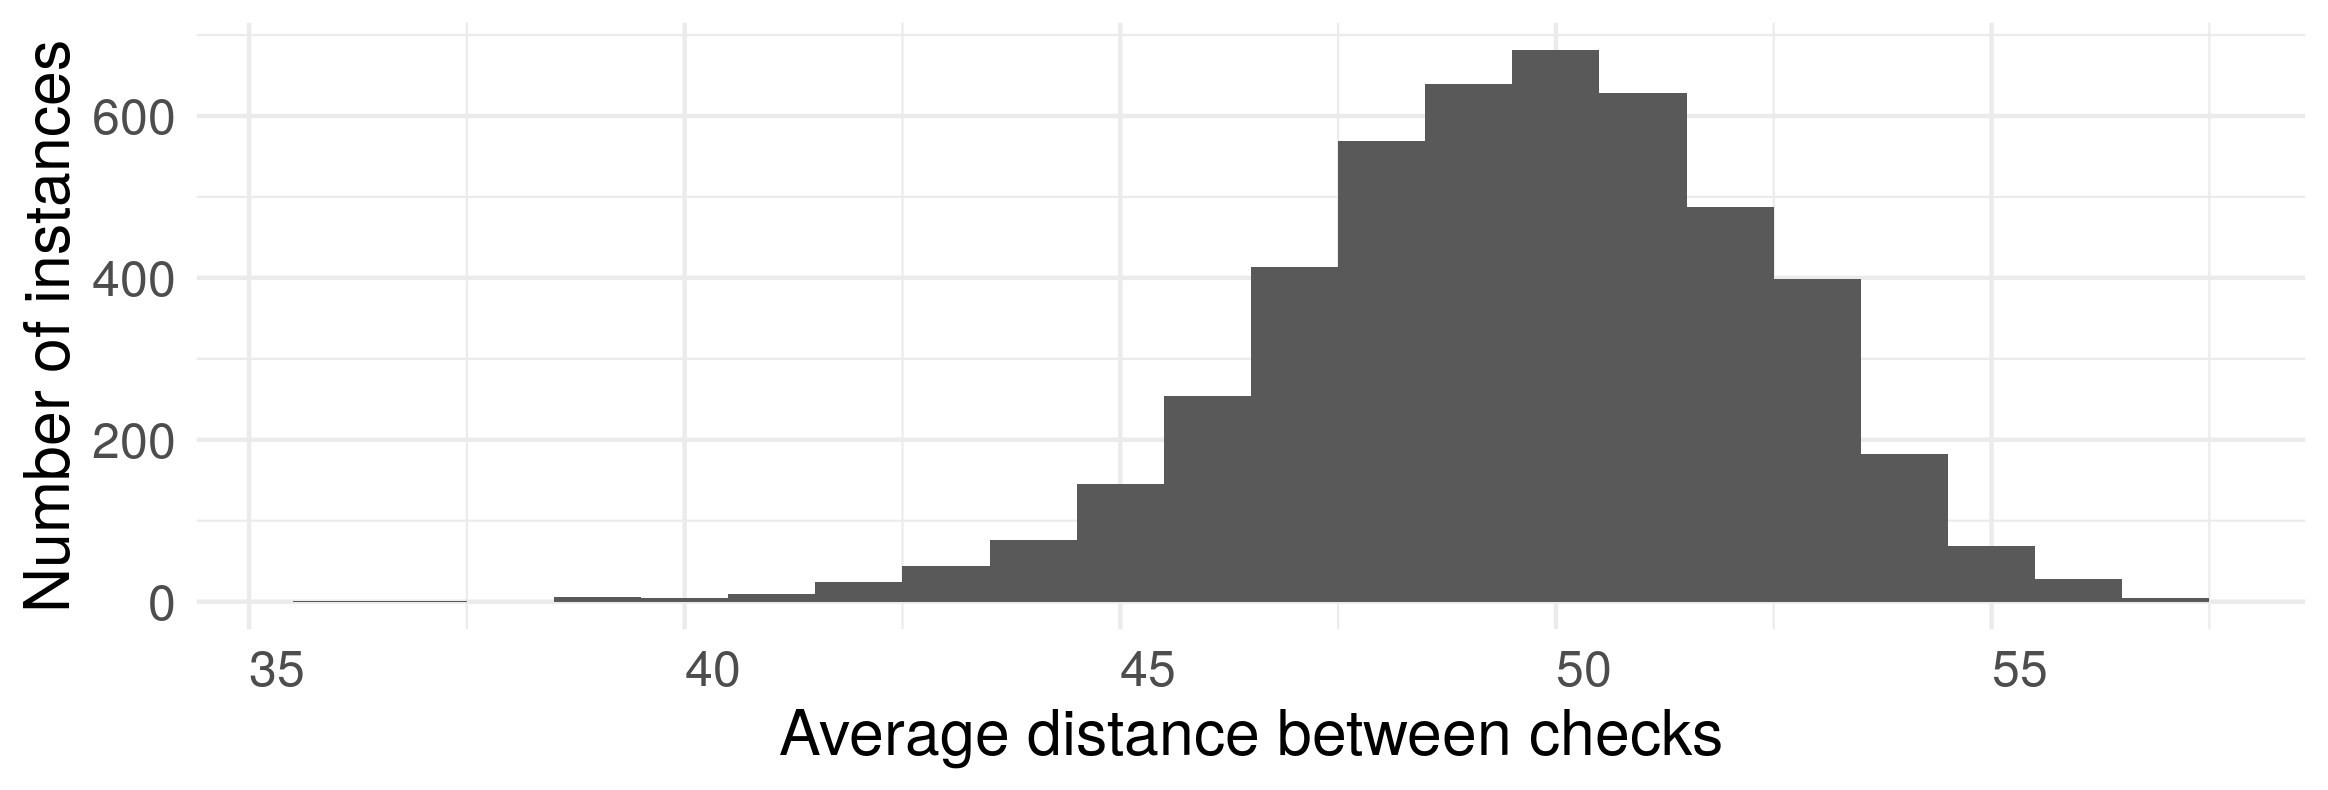
\includegraphics[height=0.4\linewidth]{images/distribution_mean_distances_IT000125_20190716}
  }
\end{frame}

\begin{frame}
\frametitle{\textbf{Solution feature prediction}}

  \begin{block}{\textbf{Technique}}
    Quantile regressions: upper bound and lower bound.
  \end{block}

  \begin{block}{\textbf{Training / test set}}
    of 5000 small instances solved to optimal and splitted: 70/30.
  \end{block}

  \begin{block}{\textbf{Input features}}
    ...
  \end{block}

  \begin{block}{\textbf{Solution features}}
    \begin{equation*}
      \mu_{t'-t} \to [\hat{\mu}_{t'-t}^{lb}, \hat{\mu}_{t'-t}^{ub}]
   \end{equation*}
  \end{block}

  % \emph{} to estimate upper and lower bounds. 
  % * \textbf{Training}: 5000 small instances. 
  % * \textbf{Input features}: 
  %   * mean flight demand per period, 
  %   * total remaining flight hours at start (init), 
  %   * variance of flight demand, 
  %   * demand of special missions, 
  %   * number of period where flight demand is cut in two. 
  % TODO: add prediction results
  % TODO: add prediction example
\end{frame}

\begin{frame}
\frametitle{\textbf{Applying learned-cuts}}

  \begin{block}{\textbf{Pattern filtering:}}
    \begin{equation*}
      D_{ip} \in [\hat{\mu}_{t'-t}^{lb} - tol, \hat{\mu}_{t'-t}^{ub} + tol] \rightarrow p \in \mathcal{P}_i 
    \end{equation*}
  \end{block}
  % TODO: add example

  \begin{block}{\textbf{Pattern recycling:} with probabiliy $\alpha$}
    \begin{equation*}
      D_{ip} \notin [\hat{\mu}_{t'-t}^{lb} - tol, \hat{\mu}_{t'-t}^{ub} + tol] \land P(\alpha)  \rightarrow p \in \mathcal{P}_i 
    \end{equation*}
  \end{block}
\end{frame}

\begin{frame}
\frametitle{\textbf{Experiments}}

  \begin{itemize}[<+->]

  \item Number of instances: medium (1000), large (1000) and very large
    (1000).
  \item Time limit at 3600 seconds.
  \item We seeded instance generation for better comparison.
  \item CPLEX running 1 thread.
  \end{itemize}

  Largest instances have 60 aircraft, 90 periods.
\end{frame}

\begin{frame}
\frametitle{\textbf{Results: performance}}

  \begin{itemize}[<+->]
    \item More solutions.
    \item Better solutions.
  \end{itemize}

  \only<1>{
    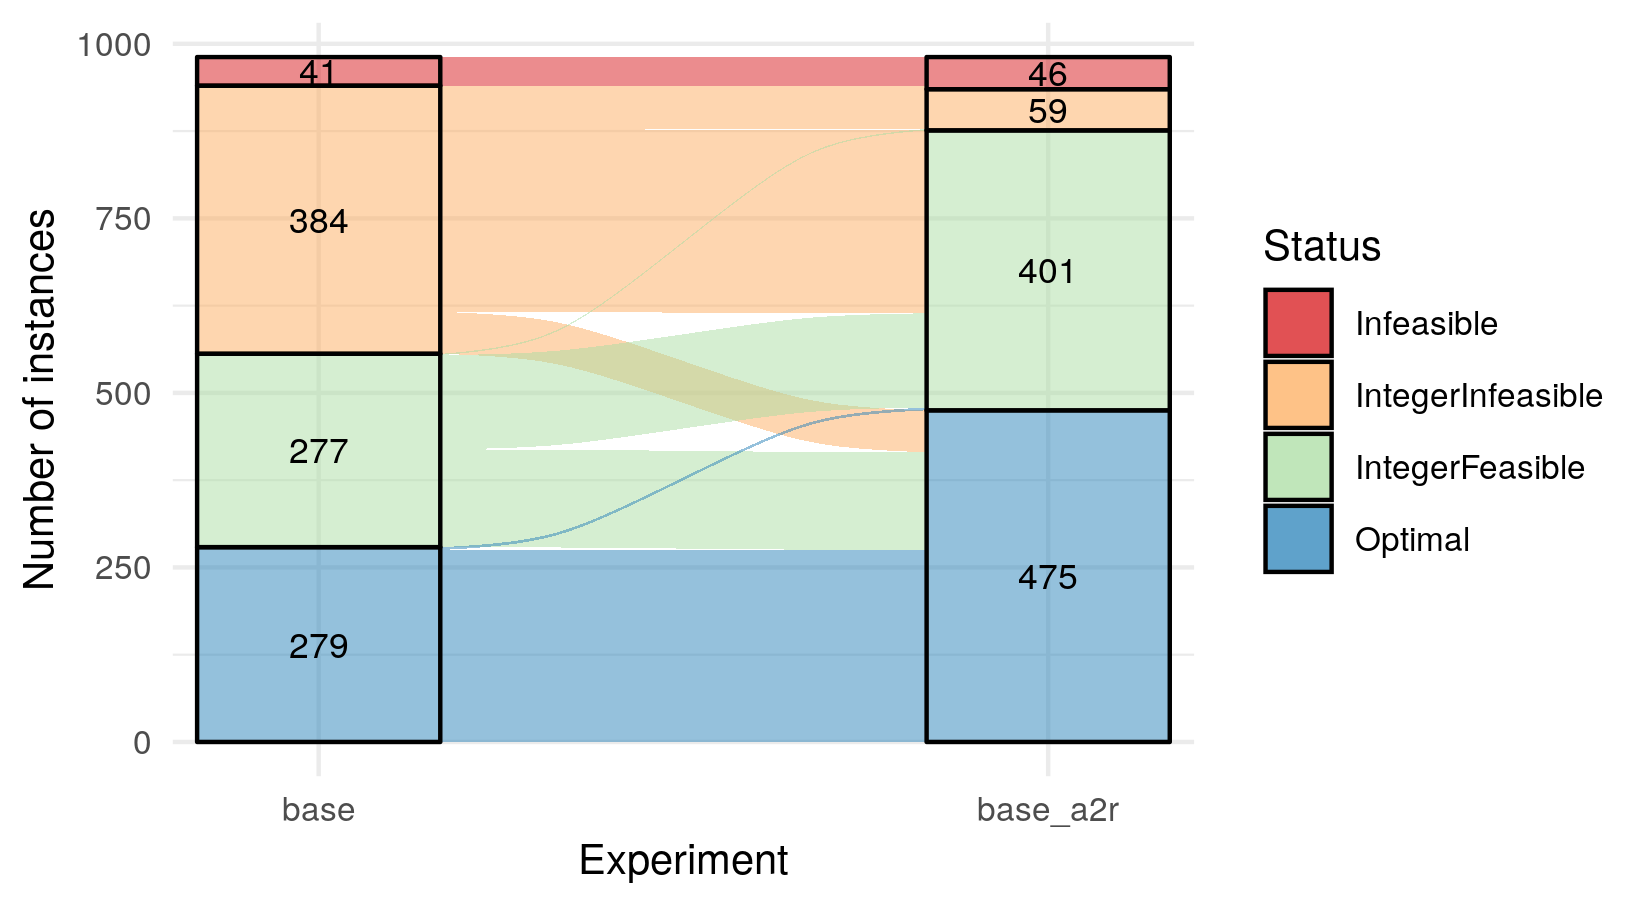
\includegraphics[width=0.8\linewidth]{images/transitions_base_2tasks.png}
  }
  \only<2>{
    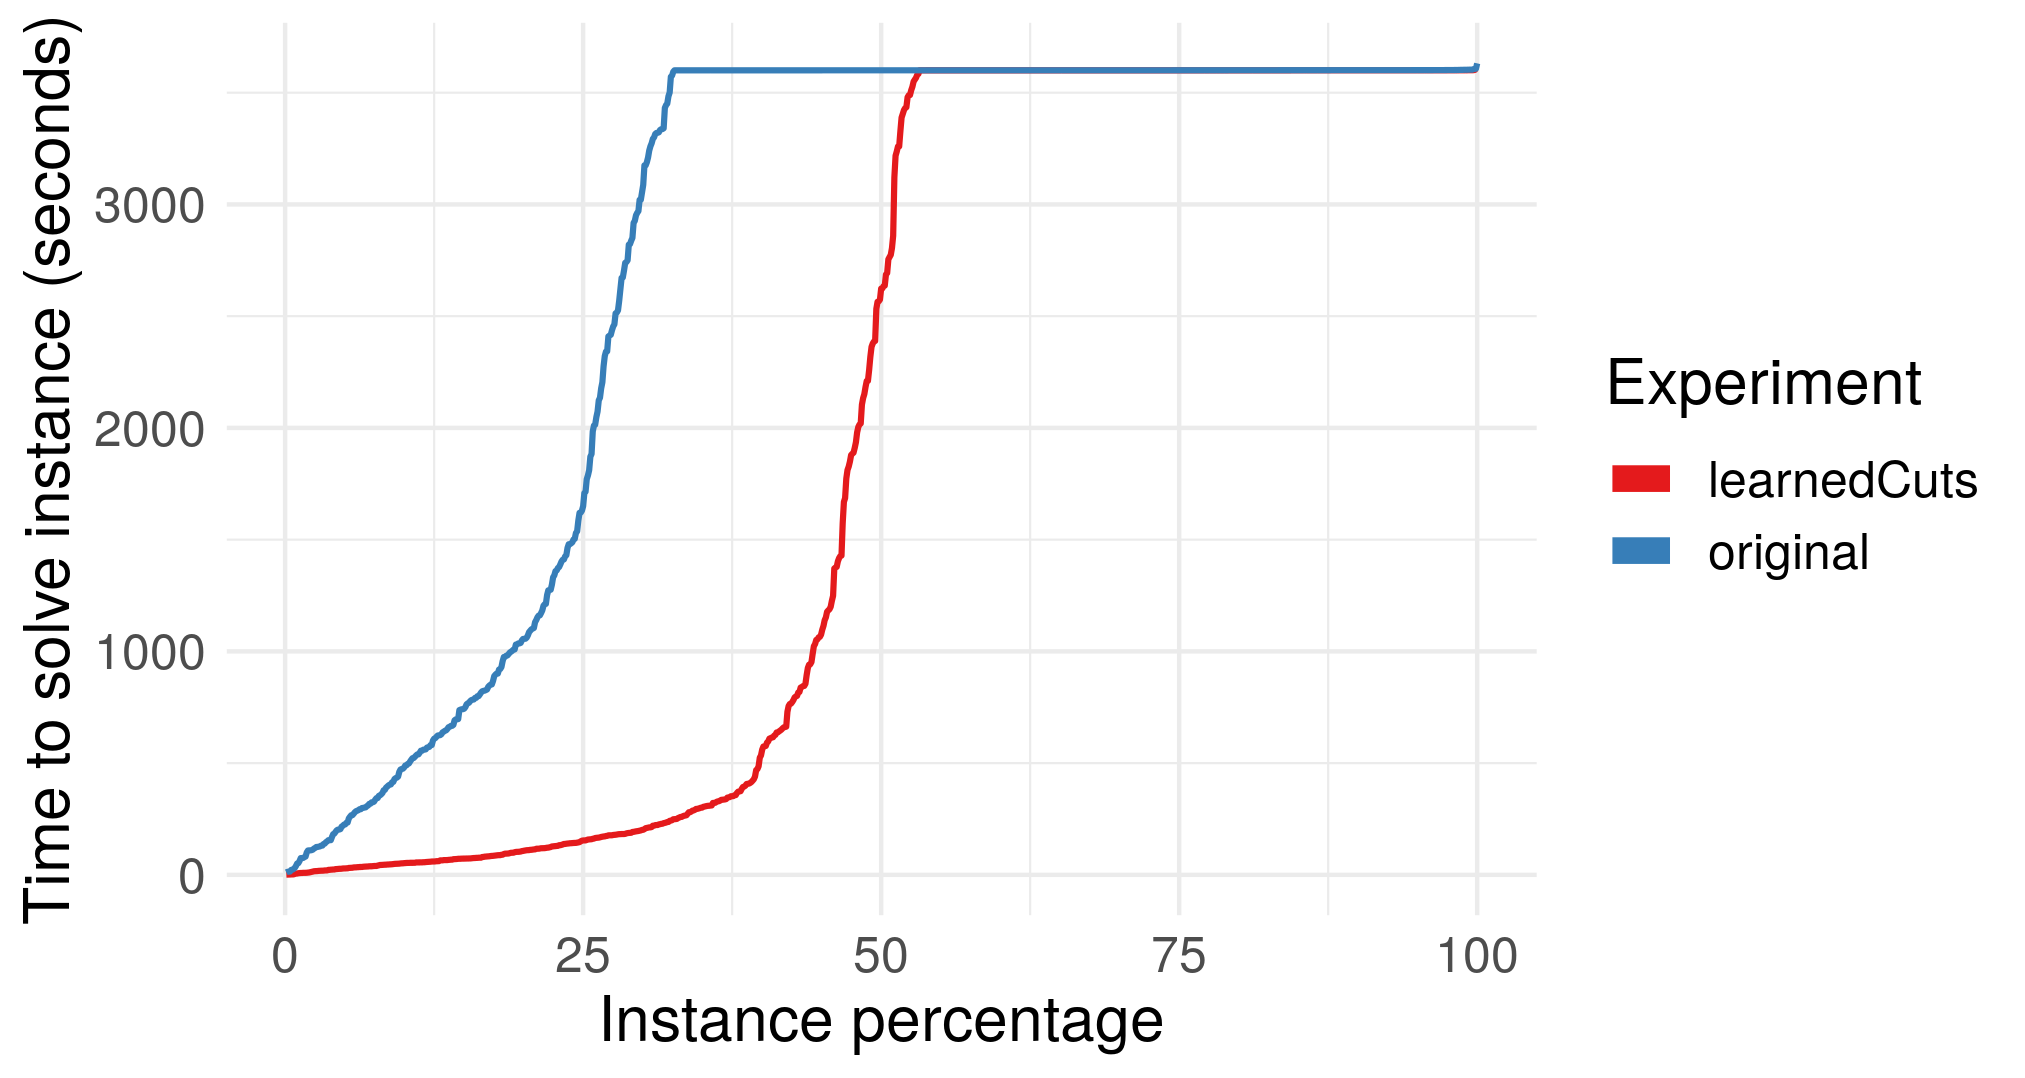
\includegraphics[width=0.8\linewidth]{images/time_performance_ordered_2tasks.png}
  }
\end{frame}

\begin{frame}
\frametitle{\textbf{Results: optimality}}

  \begin{itemize}[<+->]
    \item a < 4\% loss of optimality.
    \item better predictions can improve this.
  \end{itemize}

  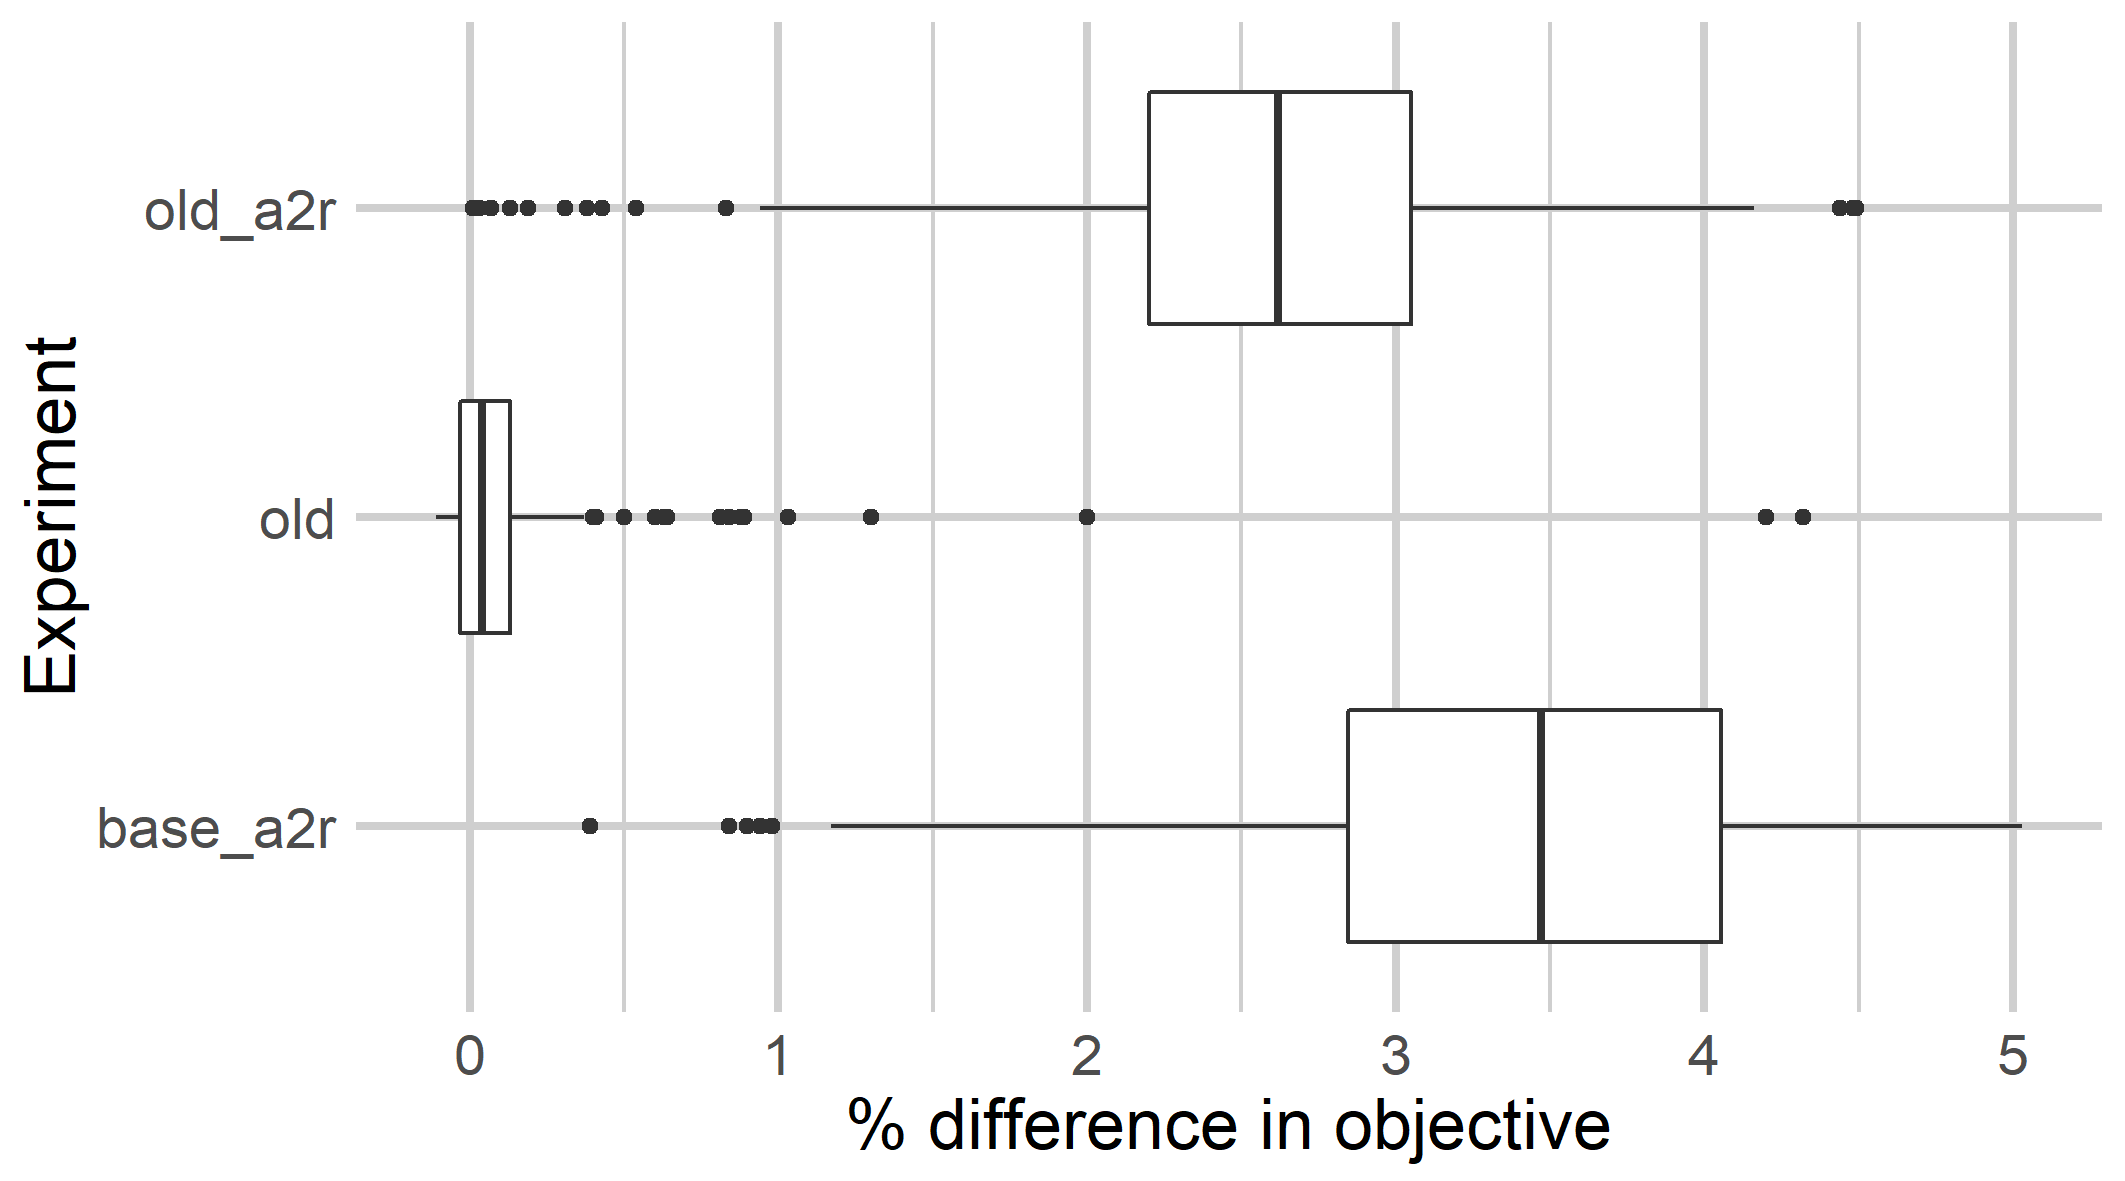
\includegraphics[width=0.8\linewidth]{images/quality_degradation_2tasks}

\end{frame}

\begin{frame}
\frametitle{\textbf{Conclusions}}
  \begin{itemize}[<+->]
  \item
    \textbf{Better predictions} with better features, or predicting
    several characteristics of optimal solutions.
  \item
    \textbf{Predict a distribution} and sample patterns from the
    distribution instead of predicting patterns.
  \item
    \textbf{Warm-start Column Generation} with a selected subset of
    potentially good patterns.
  \item
    \textbf{Automatize prediction} so it can be easily integrated in other
    problems.
  \end{itemize}
\end{frame}